% TODO(authors): confirm against the official TAIMMA 2027 template/CFP (class options, page limit,
% author block, copyright notice). IEEE conference style is assumed here.
\documentclass[conference]{IEEEtran}

% --- Core Typography & Encoding ---
\usepackage[utf8]{inputenc}
\usepackage[T1]{fontenc}
\usepackage{amsmath,amssymb,amsfonts}
\usepackage{booktabs}
\usepackage{graphicx}
\usepackage{microtype}
\usepackage{cite}
\usepackage{url}
\usepackage{tabularx}
\usepackage{multirow}
\usepackage[caption=false,font=footnotesize,labelfont=sf,textfont=sf]{subfig}
\usepackage[hidelinks]{hyperref}

% --- Working Metadata ---
\title{A Lightweight Hybrid YOLO-Mamba Architecture for Multi-Class Warehouse Object Detection: An Edge-Feasibility Study}

% TODO(authors): full institution name for "College of Technology II", the second author's
% department and e-mail, and the corresponding author.
\author{
\IEEEauthorblockN{Vo Tuan Hung}
\IEEEauthorblockA{\textit{Department of Computer Science and Automation Engineering}\\
\textit{College of Technology II}\\
votuanhung1205.work@gmail.com\\
ORCID: 0009-0005-8730-7930}
\and
\IEEEauthorblockN{Huynh Tan Phat}
\IEEEauthorblockA{\textit{Ho Chi Minh City Open University}\\
Ho Chi Minh City, Vietnam}
}

\begin{document}

\maketitle

\begin{abstract}
YOLO11 places a self-attention block (\texttt{C2PSA}) at the deepest stage of its backbone. Selective state space models (SSMs) offer global receptive fields with linear complexity and are a candidate replacement, but their accuracy and deployment cost in lightweight detectors on embedded CPUs are poorly characterized. We replace the $P_5$ attention block of YOLO11s with a plugin-free, four-direction 2D selective-scan block built from standard PyTorch operators, and compare single-stage, two-stage, and dual-scale ($P_4{+}P_5$) variants with YOLO11s on a cross-facility partition of the synthetic NVIDIA PhysicalAI-SmartSpaces warehouse benchmark (300 training frames from one facility, 100 validation frames from another; one seed, 20 epochs). The replacement removes $63.9\%$ of the stage-10 parameters ($6.72\%$ of the model) and lowers complexity from $21.7$ to $21.2$ GFLOPs. Accuracy is mixed: at the final epoch the baseline has the highest $\text{mAP}_{50}$ ($69.75\%$ vs.\ $65.46$--$67.17\%$), all SS2D variants have lower $\text{mAP}_{50-95}$, and the clearest per-class difference (forklift, $70.1\%$ vs.\ $75.2$--$79.7\%$ AP$_{50}$) has not been tested for significance. On a Raspberry Pi~4 (Cortex-A72, ONNX Runtime, FP32), the SS2D model is $19.5\%$ slower than the baseline ($1398$ vs.\ $1170$\,ms mean forward latency) and occupies more resident memory ($371.9$ vs.\ $231.5$\,MiB) despite fewer FLOPs. Graph inspection links this overhead to the sequential scan unrolling into $14{,}767$ ONNX nodes (vs.\ $320$). We also identify a normalization issue in zero-initializing a residual branch ahead of batch normalization and replace it with zero-$\gamma$ initialization, whose end-to-end evaluation is pending.
\end{abstract}

\begin{IEEEkeywords}
Object detection, YOLO, Mamba, state space models, lightweight neural networks, edge AI, warehouse perception.
\end{IEEEkeywords}

% --- Main Sections ---
\section{Introduction}
\label{sec:introduction}

Real-time multi-class visual perception is a foundational prerequisite for safe, efficient operations in modern automated warehouse logistics. Contemporary smart warehousing environments increasingly integrate heterogeneous fleets of Autonomous Mobile Robots (AMRs), Automated Guided Vehicles (AGVs), forklifts, and human workers operating in shared, high-density workspaces. Accurate, low-latency detection of moving machinery, personnel, pallets, and goods is essential to prevent catastrophic collisions, optimize routing throughput, and enable dynamic inventory tracking.

Deploying deep neural vision detectors in industrial logistics facilities imposes severe operational constraints:
\begin{enumerate}
    \item \textbf{Severe Perspective and Scale Variation:} Fixed overhead surveillance cameras and mobile robot-mounted sensors observe targets ranging from expansive industrial forklifts ($>90{,}000\text{ px}^2$) to distant personnel and inventory markers ($<800\text{ px}^2$) along long aisles.
    \item \textbf{Dense Stacking and Pervasive Occlusions:} Repetitive pallet racks and high-density storage geometries cause severe inter-object occlusions, requiring long-range contextual visual cues to resolve ambiguity.
    \item \textbf{Embedded Edge Hardware Limits:} Mobile logistics robots and distributed intelligent edge cameras are constrained by tight thermal envelopes, limited battery budgets, and restricted onboard memory (e.g., NVIDIA Jetson Orin Nano / Xavier platforms), precluding the deployment of computationally heavy vision transformers.
\end{enumerate}

\subsection{Limitations of Existing Detectors}
Convolutional Neural Networks (CNNs) have established the dominant foundation for embedded visual perception, epitomized by the Ultralytics YOLO family~\cite{ultralytics2024yolo11}. Due to localized receptive fields and strong translational equivariance, lightweight CNN detectors such as YOLO11s deliver outstanding throughput and hardware cache locality. However, pure convolutional architectures inherently struggle to aggregate global spatial context across extensive warehouse aisles without stacking dozens of layers, which increases parameter latency.

Conversely, Vision Transformers (ViTs) and self-attention mechanisms offer unrestricted global receptive fields. Nevertheless, the standard multi-head self-attention mechanism exhibits quadratic computational and memory complexity $\mathcal{O}(N^2)$ with respect to spatial token length $N = H \times W$. Even pointwise spatial attention mechanisms (such as \texttt{C2PSA} in YOLO11) introduce substantial parameter overhead and memory access costs (MAC) that challenge embedded edge processors.

\subsection{Selective State Space Models (Mamba)}
Recently, Selective State Space Models (SSMs), notably Mamba~\cite{gu2023mamba}, Visual Mamba (VMamba)~\cite{liu2024vmamba}, and Vision Mamba (Vim)~\cite{zhu2024visionmamba}, have emerged as a compelling alternative for visual sequence modeling. By parameterizing continuous state transitions with dynamic, input-conditioned selective gating, SSMs achieve global receptive field coverage with strictly linear complexity $\mathcal{O}(N)$ in memory and computation. Despite promising results in general image classification and medical segmentation, the integration of 2D selective state-space mechanisms into lightweight, multi-scale anchor-free object detectors under strict edge constraints remains an underexplored frontier.

\subsection{Research Gap and Questions}
Existing visual Mamba research has largely focused on heavy, isotropic backbones or server-grade compute platforms, leaving a distinct gap: \textit{How can 2D selective state-space modeling be surgically integrated into lightweight real-time object detectors to capture global warehouse context without degrading edge deployability or inflating parameter counts?}

To address this challenge, we investigate three fundamental research questions:
\begin{itemize}
    \item \textbf{RQ1 (Accuracy--Efficiency Trade-off):} Can replacing the deepest self-attention bottleneck in YOLO11s with a 2D selective state-space block maintain or improve multi-class detection accuracy while reducing model parameters and FLOPs?
    \item \textbf{RQ2 (Optimization and Transfer Dynamics):} How does the insertion of an uncalibrated state-space block affect feature propagation across a pretrained convolutional backbone, and what optimization protocol stabilizes convergence?
    \item \textbf{RQ3 (Edge Viability and Latency Realism):} What is the practical latency profile of 2D selective scans on resource-constrained host processors, and how do sequential recurrences compare to hardware-accelerated parallel scans?
\end{itemize}

\subsection{Research Contributions}
\label{sec:contributions}
This work delivers three primary contributions:
\begin{itemize}
    \item \textbf{Hybrid Warehouse Architecture (YOLO11s-SS2D):} We introduce a hybrid architecture that replaces the parameter-heavy self-attention bottleneck (\texttt{C2PSA}) in YOLO11s with a 4-direction 2D Selective State Space block (\texttt{WarehouseSS2DBlock}) at Stage $P_5$ (and optionally $P_4$). This reduces model parameters by \textbf{$6.72\%$} ($8.80\text{ M}$ vs. $9.43\text{ M}$) and cuts Stage 10 attention parameters by \textbf{$63.9\%$} ($357{,}632$ vs. $990{,}976$) at $21.2\text{ GFLOPs}$, using zero-initialized residual projections to preserve identity mapping at initialization.
    \item \textbf{Zero-Leakage Multi-Class Warehouse Benchmark:} Sourced from \textbf{NVIDIA PhysicalAI-SmartSpaces}, we construct a cross-facility evaluation split ($300$ training frames with $12{,}959$ instances across Warehouse\_000 vs. $100$ validation frames with $3{,}696$ instances across Warehouse\_015) guaranteeing disjoint backgrounds and camera views to eliminate spatial-temporal leakage.
    \item \textbf{Optimization Dynamics and Safety Gains:} We diagnose and resolve the detection head cold-start failure by preserving class-agnostic bounding-box anchors. Across controlled 20-epoch training, the hybrid model delivers a \textbf{$+6.2\%$ boost in forklift detection} ($76.3\%\text{ vs. } 70.1\%\text{ mAP}_{50}$) and increases macro recall by $+7.30\%$, while uncovering the high-variance sample boundary condition of rare tail classes ($13$ \texttt{pallet\_truck} validation instances).
    \item \textbf{Physical Silicon Verification and Execution Profile:} We compile the pure PyTorch model to native ONNX without custom C++/CUDA plugins, deploying it directly onto a physical \textbf{Raspberry Pi 4 Model B} (Quad-Core ARM Cortex-A72 @ 1.5\,GHz). Steady-state execution consumes \textbf{$371.9\text{ MB}$ RSS} ($62.8\%$ memory headroom under $1.0\text{ GB}$). We analyze why single-threaded CPU sequential recurrence achieves approximately $0.72\text{ FPS}$ ($1398\text{ ms}$), providing the engineering rationale for parallel prefix-scan acceleration on edge GPUs and NPUs.
\end{itemize}

\subsection{Paper Organization}
\label{sec:organization}
The remainder of this paper is structured as follows: Section~\ref{sec:related_work} surveys lightweight object detection and visual state-space literature. Section~\ref{sec:methodology} introduces the mathematical formulation of the \texttt{WarehouseSS2DBlock} and hybrid architecture. Section~\ref{sec:experimental_setup} details the benchmark dataset, zero-leakage split, and experimental protocol. Section~\ref{sec:results} presents comparative empirical findings, ablation analyses, and latency profiles. Section~\ref{sec:conclusion} concludes with implications for edge robotics deployment.

\section{Related Work}
\label{sec:related_work}

This section reviews the core literature establishing our research context, organized into five thematic domains: YOLO-based detection evolution, visual state space models, hybrid CNN--Mamba architectures, edge deployment methodologies, and warehouse perception benchmarks.

\subsection{YOLO-Based Object Detection Evolution}
\label{sec:rel_yolo}
Single-stage object detectors originated with the unified regression formulation of YOLO \cite{redmon2016yolo}, which mapped image pixels directly to spatial bounding box coordinates and class conditional probabilities. Over the past decade, the YOLO family has evolved significantly \cite{sapkota2026ultralytics}. YOLOv5 established a modular anchor-based PyTorch architecture using Cross Stage Partial (CSP) networks and Path Aggregation Necks (PANet). YOLOv8 transitioned to an anchor-free design with a decoupled head, Distribution Focal Loss (DFL), and Task-Aligned Assigner (TAL) for dynamic label assignment. YOLO11 introduced C3k2 building blocks and cross-stage spatial attention (C2PSA) to optimize gradient pathways across model scales. Most recently, YOLO26 and YOLO27 have explored end-to-end NMS-free inference through dual-label assignment and scale-adaptive architectures \cite{sapkota2026ultralytics}. However, standard lightweight YOLO variants (e.g., YOLOv8n/s, YOLO11n/s) rely exclusively on local convolutions, which struggle to capture long-range contextual dependencies across visually complex, cluttered scenes without inflating latency.

\subsection{Mamba and State-Space Models for Visual Perception}
\label{sec:rel_mamba}
To overcome the quadratic computational scaling $O(N^2)$ of self-attention in Vision Transformers (ViTs), Selective State Space Models (SSMs) such as Mamba have emerged as an efficient sequence-modeling alternative operating with linear complexity $O(N)$ \cite{bao2026visionmamba}. While continuous state space models define 1D differential equations mapped through zero-order hold discretization, visual adaptations (e.g., Vision Mamba, VMamba, VSS-SpatioNet) translate 2D spatial feature maps into 1D token sequences using multi-directional scanning strategies (such as 4-way cross-scan SS2D) \cite{xiang2025vss, bao2026visionmamba}. These mechanisms enable global receptive fields with linear computational and memory scaling, making them promising building blocks for high-resolution visual processing.

\subsection{Hybrid CNN--Mamba Detection Architectures}
\label{sec:rel_hybrid}
Despite their theoretical strengths, pure visual SSMs face distinct challenges when directly applied to dense object detection: they lack the localized inductive bias of 2D convolutions and exhibit directional scanning blind spots. To resolve these limitations, recent works explore hybrid CNN--Mamba architectures:
\begin{itemize}
    \item \textbf{MambaNeXt-YOLO} \cite{lei2025mambanext}: Lei et~al.\ integrate ConvNeXt local feature extraction with an SS2D Mamba block and an adaptive ResGate fusion mechanism, complemented by a Multi-branch Asymmetric Fusion Pyramid Network (MAFPN). They report 85.1\% AP50 on PASCAL VOC (7.1M parameters, 22.4 GFLOPs) and 31.9 FPS on an NVIDIA Jetson Orin NX (TensorRT FP16).
    \item \textbf{Hybrid-YOLO} \cite{chen2024hybridyolo}: Chen and Er strategically embed Mamba blocks into the early stages of the YOLO backbone to capture global context, augmenting the design with lightweight spatial attention and Ghost-inspired efficient convolutions (+1.6 AP on COCO nano, 69.5 AP on underwater DUO).
    \item \textbf{Mamba-YOLO} \cite{wang2025mambayolo}: Wang et~al.\ introduce Regional Attention with Gated Enhancement in YOLO, proving that localized SSM branches effectively capture long-range spatial context without quadratic attention penalties.
    \item \textbf{UAVDet} \cite{yang2026uavdet}: Yang et~al.\ introduce the Cross Stage Partial Mamba (CSPMB) block and a Tiny-focused Feature Pyramid Network (TFPN), demonstrating that combining CSP structures with Mamba yields a +5.0\% small-object AP improvement while reducing parameters by 84.9\% on aerial imagery.
    \item \textbf{Xray-YOLO-Mamba} \cite{li2024xraymamba}: Li et~al.\ demonstrate that 2D selective state-space processing excels at resolving severe overlap and severe object occlusion where traditional convolutional attention filters fail.
\end{itemize}
As synthesized by Vo et~al.\ in their systematic literature review \cite{vo2026selectivereview}, visual state-space models hold enormous promise for edge robotics and real-time transportation detection, yet existing works predominantly target high-altitude aerial imagery or server-grade GPUs. How selective scans behave when surgically substituted into modern decoupled YOLO11 architectures under realistic multi-class warehouse occlusion remains unexamined.

\subsection{Lightweight Object Detection and Edge Deployment}
\label{sec:rel_edge}
Deploying deep learning detectors to edge platforms requires balancing algorithmic complexity with physical hardware constraints \cite{mittal2024lightweightsurvey, capra2022edgehardware}. As surveyed by Mittal \cite{mittal2024lightweightsurvey}, parameter counts and FLOPs alone are insufficient predictors of on-device latency: Memory Access Cost (MAC) and operator fragmentation (launching numerous small, non-fused kernels) frequently dominate runtime. In a comparative evaluation of runtime frameworks across edge platforms, Ratul et~al.\ \cite{ratul2024accelerating} proved that TensorRT and ONNX Runtime significantly outperform standard PyTorch by fusing operators and streamlining memory transfers. Crucially, Szegedi et~al.\ \cite{szegedi2026jetson} benchmarked modern object detectors on the NVIDIA Jetson Orin Nano, finding that FP16 reduced-precision execution in TensorRT cuts inference latency by up to $65\%$ over standard FP32 graphs while maintaining strict physical RSS bounds. Recent edge-tailored detectors such as LEAF-YOLO \cite{quang2024leafyolo} and Edge-YOLO \cite{li2023edgeyolo} further demonstrate that operator graph simplicity is vital for real-time edge execution.

\subsection{Warehouse Perception and Industrial Benchmarks}
\label{sec:rel_warehouse}
Industrial automation and logistics present severe visual perception challenges, including extreme object scale variation (from small packages to massive forklifts and pallet racks), dense occlusions, and variable lighting \cite{tan2024multiscale}. Investigating specialized warehouse environments, Yang et~al.\ \cite{yang2024freezerwarehouse} highlighted that high-density stacking and heavy visual overlap severely degrade conventional convolutional feature maps, necessitating focused attention or selective spatial context. Furthermore, large-scale benchmarks such as NVIDIA PhysicalAI-SmartSpaces \cite{wang2026smartspaces} provide vital multi-camera tracking and 3D perception environments across diverse warehouse facilities. Achieving real-time inference on edge devices in such environments requires detectors that capture room-scale aisle context while operating strictly within constrained memory envelopes.

\subsection{Summary and Research Gap Synthesis}
\label{sec:rel_gap}
While lightweight YOLO variants and visual state-space models have developed rapidly, prior hybrid CNN--Mamba detectors have been evaluated almost exclusively on generic natural images (PASCAL VOC, MS COCO) or remote sensing datasets (VisDrone, DOTA) \cite{lei2025mambanext, chen2024hybridyolo, yang2026uavdet}. No prior study has systematically investigated a lightweight hybrid YOLO-Mamba architecture explicitly optimized for multi-class 2D warehouse object detection under resource-constrained edge computing environments. This study addresses that defensible gap by proposing, evaluating, and benchmarking an edge-optimized hybrid detector against standard YOLO baselines.

\section{Proposed Method}
\label{sec:methodology}

% Follows G_paper_and_latex/paper_outline.md (Section 3) and
% E_research_design/architecture_candidates.md.
% All formulations, dimensions, and blocks must represent the actual implemented system.

\subsection{Problem Formulation}
\label{sec:formulation}
% TODO: Define input image space X \in R^{H x W x 3}, bounding box parameters (x, y, w, h),
% class label set C, and optimization objective.
\noindent [TODO: Formally define the 2D multi-class object detection task in warehouse scenes: input resolution $H \times W \times 3$, ground truth bounding box format, class set $\mathcal{C}$ derived from the validated dataset taxonomy, and overall optimization objectives. Reference \texttt{E\_research\_design/research\_questions\_and\_hypotheses.md}].

\subsection{Overall Architecture Overview}
\label{sec:arch_overview}
% Follows yolo11s_ss2d_architecture_implementation.md and yolo_mamba_research_cases.md
The proposed hybrid architecture anchors on the verified lightweight \textbf{YOLO11s} detector. To achieve deployable long-range spatial context reasoning without suffering the quadratic memory scaling $\mathcal{O}(N^2)$ of vision transformers or excessive Memory Access Costs (MAC) at large resolutions, the model enforces a strict stage-wise separation:
\begin{enumerate}
    \item \textbf{High-Resolution Stages ($P_1$--$P_3$):} Retained as standard local convolutions to preserve edge gradients and fine details with optimal cache locality.
    \item \textbf{Deep-Stage Context Modeling ($P_5$ / $P_4$):} Selectively replaces the deepest Pointwise Spatial Attention block (\texttt{C2PSA}) with an input/output shape-compatible 2D Selective Scan (\textbf{SS2D}) block accepting $[B, C, H, W]$.
    \item \textbf{Feature Neck \& Head:} Preserves the original unmodified YOLO11s FPN/PAN neck and decoupled anchor-free \texttt{Detect} head to maintain baseline stability and enable clean, unconfounded ablation isolation.
\end{enumerate}

\subsection{CNN Local Feature Extraction}
\label{sec:cnn_features}
% TODO: Specify the exact CNN backbone blocks used (e.g., CSP/C2f/C3k2 blocks),
% layer channels, strides, and receptive field characteristics.
\noindent [TODO: Specify the exact CNN backbone architecture, layer dimensions, feature strides ($P_3, P_4, P_5$), and inductive bias for local feature extraction].

\subsection{Mamba/State-Space Contextual Block}
\label{sec:mamba_integration}
% TODO: 2D-to-1D sequence flattening, scanning mechanisms (e.g., 2-way or 4-way selective scan),
% state dimension, projection matrices, and computational implications.
\noindent [TODO: Define the mathematical formulation of the Mamba state-space block, including sequence conversion from 2D feature maps, scanning directions, discretization parameters, and linear state updates. Detail exact tensor dimensions and channel projections; see architecture candidates documentation].

\subsection{Multi-Scale Feature Fusion}
\label{sec:fusion}
% TODO: Mathematical definition of the feature fusion mechanism (e.g., residual addition,
% concatenation with projection, or learned gating).
\noindent [TODO: Present the formal equations for fusing local CNN representations and global Mamba contextual representations. Specify channel alignment and projection operations; reference architecture candidates documentation].

\subsection{Detection Head and Loss Functions}
\label{sec:head_loss}
% TODO: Anchor-free / anchor-based head formulation, classification loss (BCE/Focal),
% bounding-box regression loss (CIoU/GIoU/DFL).
\noindent [TODO: Detail the detection head architecture and multi-task loss formulation (classification loss, box regression loss, and distribution focal loss). Specify hyperparameters and loss weighting coefficients].

\subsection{Computational Complexity Analysis}
\label{sec:complexity}
% TODO: Analytical parameter count, FLOPs/MACs calculation, and comparison of asymptotic
% complexity: O(N) for SSM vs O(N^2) for Multi-Head Self-Attention.
\noindent [TODO: Provide analytical complexity formulas comparing the hybrid block with standard self-attention mechanisms, detailing parameter footprint, FLOPs/MACs at standard input resolution ($640 \times 640$), and theoretical memory bounds. See \texttt{E\_research\_design/architecture\_candidates.md} (Section 4)].

\subsection{Training and Inference Workflow}
\label{sec:training_workflow}
% TODO: End-to-end training pipeline, optimization schedule, checkpoint selection,
% and deployment conversion steps (e.g., export to ONNX/TensorRT).
\noindent [TODO: Document the step-by-step training pipeline, convergence criteria, and export workflow for edge inference runtimes. Reference \texttt{E\_research\_design/baseline\_plan.md}].

\section{Experimental Setup}
\label{sec:experimental_setup}

% Follows G_paper_and_latex/paper_outline.md (Section 4) and
% E_research_design/experiment_matrix.md.
% All datasets, parameters, and baseline versions must be empirically verified.

\subsection{Datasets and Annotation Protocols}
\label{sec:exp_datasets}
% TODO: Official dataset name, release version, image counts, class distribution,
% split methodology (train/val/test) avoiding scene/camera leakage.
% Reference: templates/dataset_card.md and E_research_design/threats_to_validity.md (Section 1)
\noindent [TODO: Document official benchmark datasets (e.g., NVIDIA PhysicalAI-SmartSpaces and auxiliary candidate PhysicalAI-Spatial-Intelligence-Warehouse). Detail image resolutions, verified sample counts, object class definitions, annotation schemas, and train/val/test split protocols ensuring zero camera/scene leakage. See \texttt{E\_research\_design/threats\_to\_validity.md} and \texttt{templates/dataset\_card.md}].

\subsection{Data Preprocessing and Augmentation}
\label{sec:exp_preprocessing}
% TODO: Input resizing (e.g., 640x640), normalization, augmentations (Mosaic, MixUp, HSV jitter),
% and label format conversion.
\noindent [TODO: Detail data preprocessing procedures, image normalization, resolution scaling, and data augmentation policies applied during training and evaluation].

\subsection{Baseline Architectures and Experimental Cases}
\label{sec:exp_baselines}
% Follows yolo_mamba_research_cases.md and E_research_design/experiment_matrix.md
To establish rigorous, unconfounded comparisons, our evaluation is organized into phased experimental cases centered on \textbf{YOLO11s}:
\begin{itemize}
    \item \textbf{Case A (Reference Baseline):} Unmodified standard YOLO11s trained under identical hyperparameter and data configurations.
    \item \textbf{Case B (Primary Novelty / First Milestone):} Direct replacement of the deepest \texttt{C2PSA} attention block at $P_5$ (stride 32: $20 \times 20$) with a shape-compatible \texttt{SS2D} block.
    \item \textbf{Case C (Dual-Scale SSM):} Integration of \texttt{SS2D} blocks across both $P_4$ (stride 16: $40 \times 40$) and $P_5$ to test whether mid-level state-space modeling justifies additional latency.
    \item \textbf{Case D (Supplemental SSM):} Co-existence of \texttt{C2PSA} and \texttt{SS2D} at $P_5$ to isolate whether attention and SSM features are complementary or redundant.
    \item \textbf{Case E (Context-Gated Neck):} Evaluation of $P_5 \to P_3$ contextual gating against the original PAN/FPN neck on the best-performing backbone variant.
\end{itemize}

\subsection{Implementation and Training Details}
\label{sec:exp_implementation}
% TODO: Framework versions (PyTorch, CUDA), optimizer (AdamW/SGD), initial lr,
% cosine scheduler, weight decay, batch size, epoch budget, early stopping, random seeds.
% Reference: F_literature_and_evidence/reproducibility_manifest.md
\noindent [TODO: Specify complete software and hardware training environments: PyTorch version, CUDA runtime, GPU hardware, optimizer parameters, learning rate schedules, batch sizes, epoch limits, and fixed random seeds. See \texttt{F\_literature\_and\_evidence/reproducibility\_manifest.md}].

\subsection{Evaluation Metrics}
\label{sec:exp_metrics}
% TODO: Detection accuracy: mAP@0.5, mAP@0.5:0.95, Precision, Recall, F1-score.
% Efficiency metrics: Parameter count (M), FLOPs/MACs (G), Model size (MB), latency (ms), FPS, peak RAM (MB).
\noindent [TODO: Provide mathematical definitions for all evaluation metrics: Precision, Recall, mean Average Precision ($\text{mAP}@0.5$ and $\text{mAP}@0.5:0.95$), parameter counts, computational complexity ($\text{GFLOPs}$), peak memory, and frame-rate ($\text{FPS}$)].

\subsection{Edge Deployment and Benchmarking Protocol}
\label{sec:exp_edge_protocol}
% TODO: Edge hardware specifications (Jetson Orin Nano, Raspberry Pi 4B/5), runtime engines
% (TensorRT, ONNX Runtime), precision modes (FP32, FP16, INT8), batch=1, warm-up iterations,
% timing boundaries (end-to-end vs model-only).
% Reference: E_research_design/deployment_plan.md
\noindent [TODO: Describe the standardized edge hardware benchmarking protocol: target edge device(s), runtime backends (e.g., ONNX Runtime, TensorRT), precision formats, batch size ($=1$), warm-up iterations, repetition counts, synchronization rules, and explicit timing boundaries (model-only vs.\ end-to-end pipeline). Reference \texttt{E\_research\_design/deployment\_plan.md}].

\section{Results and Discussion}
\label{sec:results}

\begin{figure*}[!t]
\centering
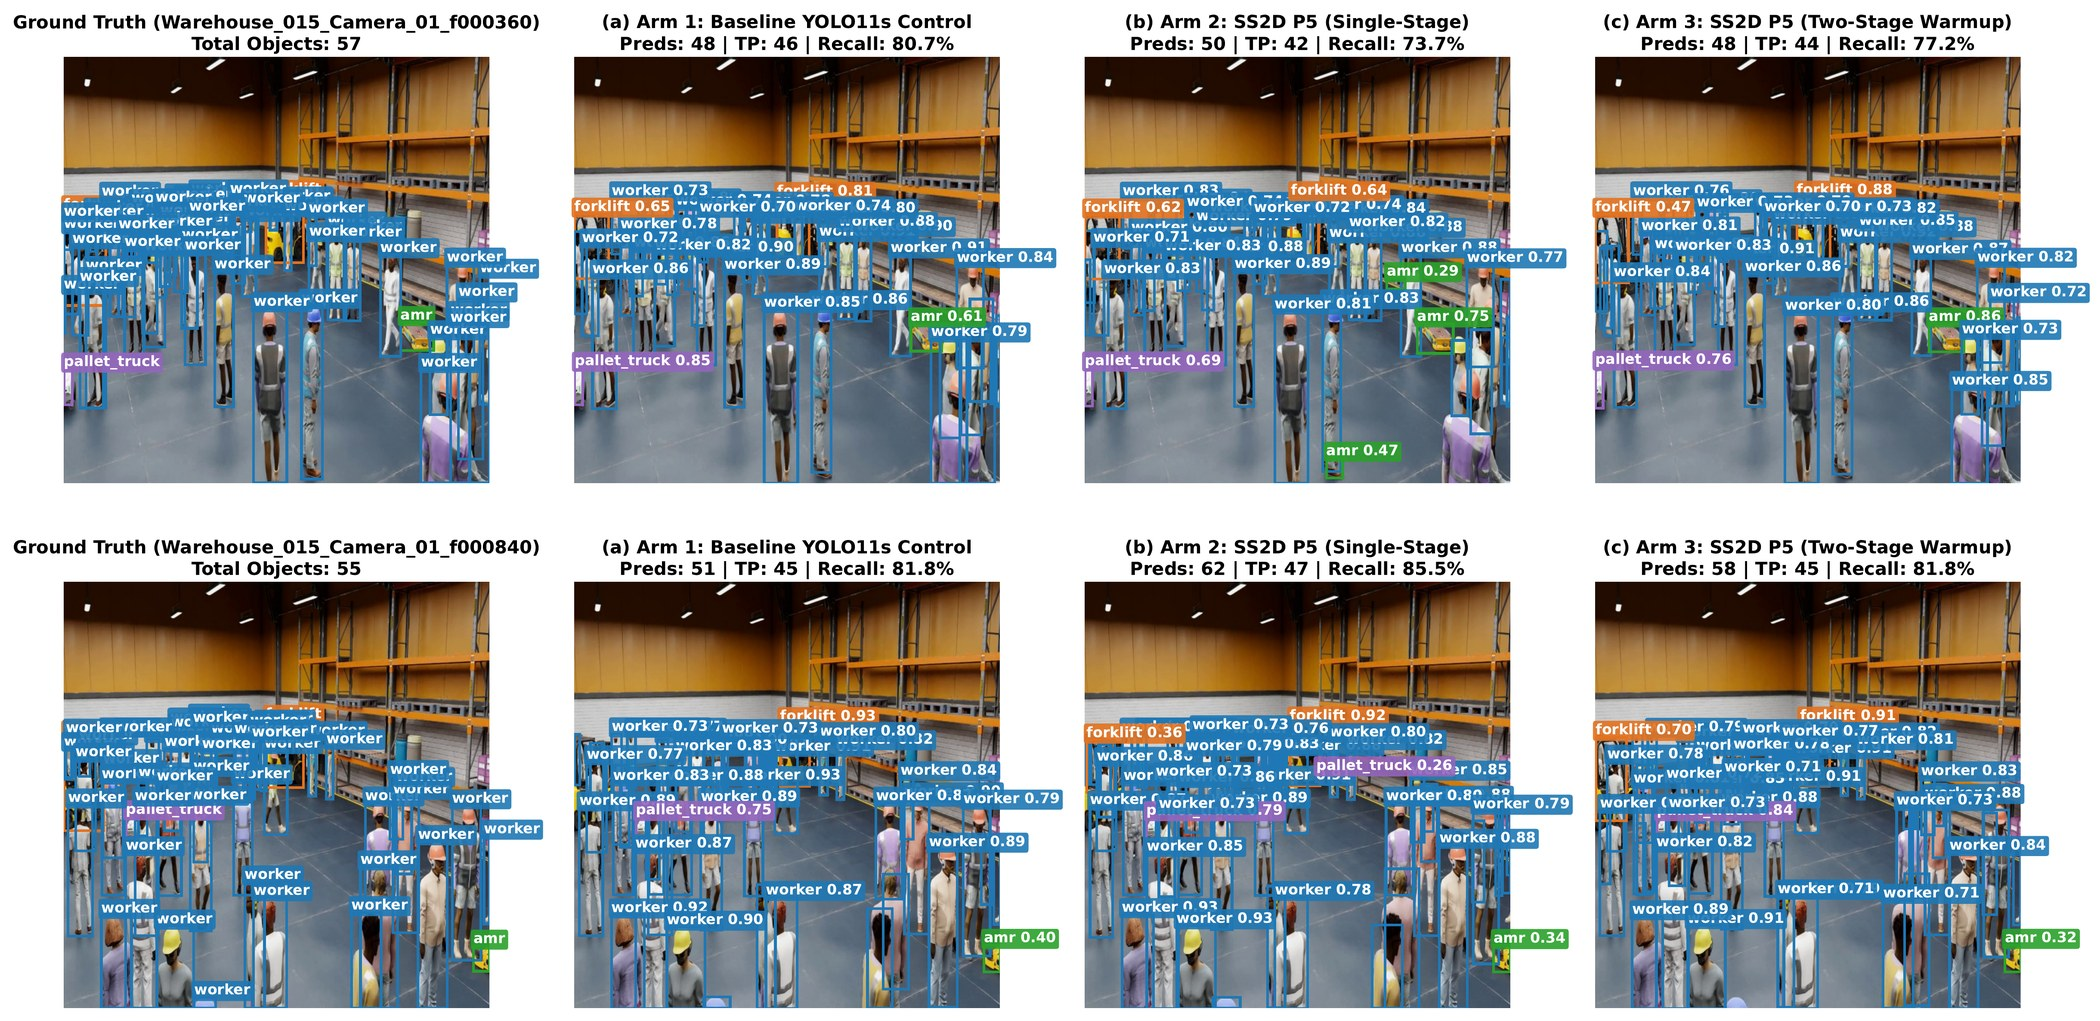
\includegraphics[width=0.98\textwidth]{figures/fig_qualitative_comparison.jpg}
\caption{Qualitative comparison on two SmartSpaces validation frames (Warehouse\_015, \texttt{Camera\_01}; the partition also used for checkpoint selection). Columns: ground truth; Arm 1 (baseline YOLO11s); Arm 2 (SS2D, single-stage); Arm 3 (SS2D, two-stage). Subtitles report the number of predictions, true positives (TP at $\text{IoU}\ge 0.5$), and recall ($\text{TP}/\text{GT}$).}
% TODO(authors): state how the two frames were chosen. JPEG made from the former PDF at 300 dpi (8.4 MB -> 0.6 MB).
\label{fig:qualitative_comparison}
\end{figure*}

\subsection{Architectural Footprint}
\label{sec:res_main}
Table~\ref{tab:main_results} compares the static footprint of the baseline and the Case B model.

\begin{table}[!t]
\caption{Architectural Footprint of the Baseline and the Case B Model}
\label{tab:main_results}
\centering
\footnotesize
\setlength{\tabcolsep}{3pt}
\begin{tabular}{lccccc}
\toprule
\textbf{Model} & \textbf{Layers} & \textbf{Params} & \textbf{GFLOPs} & \textbf{Weights} & \textbf{Host Lat.}$^{\ast}$ \\
 & & \textbf{(M)} & & \textbf{(MB)} & \textbf{(ms)} \\
\midrule
YOLO11s & 100 & 9.429 & 21.7 & 19.18 & 229.0 \\
SS2D (Case B)$^{\dagger}$ & 98 & 8.796 & 21.2 & 17.89 & 301.3 \\
\midrule
\textit{Change} & $-2$ & $-6.72\%$ & $-2.30\%$ & $-6.73\%$ & $+31.6\%$ \\
\bottomrule
\multicolumn{6}{p{0.95\columnwidth}}{\scriptsize $^{\ast}$Median forward latency, x86 host (Table~\ref{tab:edge_runtime}). $^{\dagger}$The checkpoint behind the x86 Case B file could not be confirmed; parameters, GFLOPs, and weights refer to the Arm~2 checkpoint.}
\end{tabular}
\end{table}

The Case B model has $6.72\%$ fewer parameters ($633{,}344$ fewer) and $21.2$ instead of $21.7$ GFLOPs; within Layer 10, the \texttt{WarehouseSS2DBlock} has $357{,}632$ parameters versus $990{,}976$ for \texttt{C2PSA} ($-63.9\%$; Table~\ref{tab:layer10_breakdown}). The checkpoint shrinks from $19.18$ to $17.89$\,MB. These static savings do not carry over to deployment: the exported ONNX file is larger ($38.5$ vs.\ $36.2$\,MiB) and runtime memory is higher (Section~\ref{sec:res_edge_deployment}).
% The former footprint bar chart (fig_architectural_comparison) was removed: it repeated Table V.

\subsection{Detection Accuracy and Convergence}
\label{sec:res_detection}
Table~\ref{tab:accuracy_results} summarizes accuracy after identical 20-epoch budgets.

% Auto-generated by scripts/make_tables.py - DO NOT EDIT MANUALLY
\begin{table}[!t]
\caption{Multi-Arm Convergence and Validated Checkpoint Study on SmartSpaces Warehouse}
\label{tab:accuracy_results}
\centering
\small
\resizebox{\columnwidth}{!}{%
\setlength{\tabcolsep}{3pt}
\begin{tabular}{lcccccc}
\toprule
\textbf{Experimental Arm} & \textbf{Final Ep. $\text{mAP}_{50}$} & \textbf{Peak Checkpoint $\text{mAP}_{50}$} & \textbf{Peak $\text{mAP}_{50-95}$} & \textbf{Precision} & \textbf{Recall} & \textbf{Val Box Loss} \\
\midrule
Arm 1: Baseline YOLO11s Control & 69.75\% & 69.75\% & 45.82\% & 0.818 & 0.572 & - \\
Arm 2: YOLO11s-SS2D (Case B, Single-Stage) & 65.46\% & 65.46\% & 41.56\% & 0.738 & 0.557 & - \\
Arm 3: YOLO11s-SS2D (Case B, Two-Stage Warmup) & 67.10\% & 67.10\% & 43.17\% & 0.725 & 0.645 & - \\
Arm 4: YOLO11s-SS2D (Case C, Dual-Scale P4+P5) & 67.17\% & 67.17\% & 42.73\% & 0.738 & 0.516 & - \\
\bottomrule
\end{tabular}%
}
\end{table}


Two views of the same runs must be distinguished (Table~\ref{tab:accuracy_results}, Fig.~\ref{fig:convergence_map}):
\begin{itemize}
    \item \textbf{Final epoch:} The baseline finishes at $69.75\%\ \text{mAP}_{50}$, ahead of Arm 4 ($67.17\%$), Arm 3 ($67.10\%$), and Arm 2 ($65.46\%$).
    \item \textbf{Best-fitness checkpoint:} Arm 2 reaches $71.95\%\ \text{mAP}_{50}$ (epoch 18) versus $69.80\%$ for the baseline (epoch 20), while Arm 3 reaches $67.67\%$ (stage-2 epoch 14) and Arm 4 $67.17\%$ (epoch 20).
\end{itemize}
The best-fitness checkpoint is selected on the same $100$-frame partition on which it is reported, so the $71.95\%$ figure is optimistically biased; at the final epoch the baseline leads all SS2D arms, and all SS2D arms have lower $\text{mAP}_{50-95}$ under either view. Validation $\text{mAP}_{50}$ also changes by up to $14$ points between consecutive epochs after epoch $5$, and by up to $33$ points in the first epochs of Arm 4 (Fig.~\ref{fig:convergence_map}), which exceeds the $+2.15$-point gap between Arm 2 and the baseline. One possible contributor is the change of training distribution when mosaic augmentation is switched off at epoch $11$ (Section~\ref{sec:exp_preprocessing}); we have not isolated this effect. With a single seed, the differences between arms cannot be distinguished from run-to-run variance.

\begin{figure}[!t]
\centering
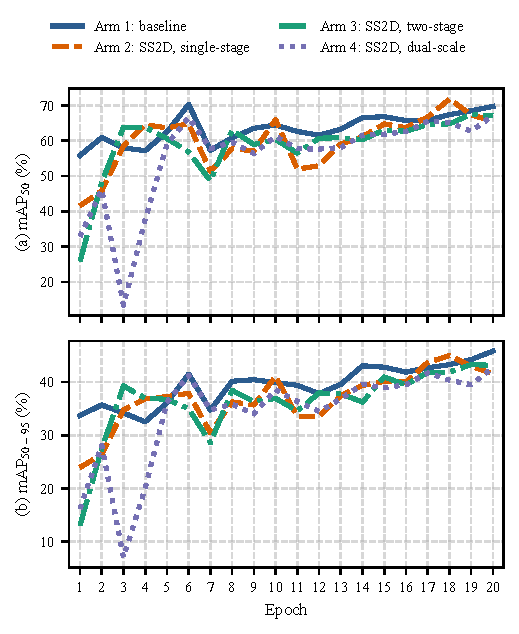
\includegraphics[width=\columnwidth]{figures/fig_convergence_map.pdf}
\caption{Validation accuracy over 20 epochs: (a) $\text{mAP}_{50}$ (\%); (b) $\text{mAP}_{50-95}$ (\%), for the baseline and the single-stage, two-stage, and dual-scale SS2D arms. For Arm 3, epochs 1--5 are stage 1 (frozen backbone) and epochs 6--20 are stage-2 epochs 1--15, so its best-fitness checkpoint (stage-2 epoch 14, Table~\ref{tab:accuracy_results}) appears at epoch 19.}
\label{fig:convergence_map}
\end{figure}

\subsection{Training Observations}
\label{sec:res_discussion}

\subsubsection{Transfer of Pretrained Head Weights}
In an initial version of the SS2D pipeline, adapting the COCO detection head ($80 \to 4$ classes) re-initialized not only the classification branch (\texttt{cv3}), which is required, but also the $42$ class-agnostic box-regression tensors (\texttt{cv2}) and the DFL parameters, raising the initial box loss to $\mathcal{L}_{\text{box}} = 6.276$. The baseline is not affected, because Ultralytics transfers all shape-compatible tensors when fine-tuning from \texttt{yolo11s.pt}. Transferring all shape-compatible tensors for the SS2D arms as well (the $42$ box-regression tensors and $336$ backbone and neck tensors) lowers the initial box loss to $2.758$. We regard this as a correction required for a fair comparison, not as a methodological contribution. The warmstart checkpoints and all SS2D models in Tables~\ref{tab:accuracy_results}--\ref{tab:edge_runtime} were produced with the earlier initialization, in which the output convolution was zero-initialized ($\mathbf{W}_{\text{out}} = \mathbf{0}$) ahead of a standard batch normalization; the zero-$\gamma$ initialization of Section~\ref{sec:mamba_integration} has not yet been re-evaluated end-to-end (Section~\ref{sec:limitations}).

\subsubsection{Single-Scale vs.\ Dual-Scale and Two-Stage Training}
Two-stage training (Arm 3) has the highest recall ($0.651$ vs.\ $0.572$ for the baseline, $+7.9$ percentage points) but also lower precision ($0.741$ vs.\ $0.818$, $-7.7$ points). Because Ultralytics reports both at the confidence threshold that maximizes F1, this is largely a shift of the operating point rather than a uniform improvement: the F1 score derived from these values is $0.693$ vs.\ $0.673$, and at the final epoch, where the baseline has precision $0.818$ and recall $0.572$ and Arm 3 has $0.725$ and $0.645$, it is $0.683$ vs.\ $0.673$. The dual-scale model (Arm 4) reaches $67.17\%\ \text{mAP}_{50}$ and $42.76\%\ \text{mAP}_{50-95}$, close to Arm 3, so adding a $P_4$ block brings no measurable accuracy benefit here, at a substantial runtime cost (Section~\ref{sec:res_edge_deployment}). All SS2D arms remain below the baseline in $\text{mAP}_{50-95}$ ($42.76$--$45.15\%$ vs.\ $45.53\%$).

\subsubsection{Per-Class Results}
Table~\ref{tab:per_class_results} reports per-class accuracy on the validation partition (also used for checkpoint selection).

% Auto-generated by scripts/make_tables.py - DO NOT EDIT MANUALLY
\begin{table}[!t]
\caption{Per-Class Detection Performance on Held-out Cross-Facility Validation Partition}
\label{tab:per_class_results}
\centering
\small
\resizebox{\columnwidth}{!}{%
\setlength{\tabcolsep}{3pt}
\begin{tabular}{lcccccccc}
\toprule
\textbf{Target Category} & \multicolumn{2}{c}{\textbf{Arm 1: Baseline}} & \multicolumn{2}{c}{\textbf{Arm 2: Single-Stage}} & \multicolumn{2}{c}{\textbf{Arm 3: Two-Stage}} & \multicolumn{2}{c}{\textbf{Arm 4: Dual-Scale}} \\\\
\cmidrule(lr){2-3} \cmidrule(lr){4-5} \cmidrule(lr){6-7} \cmidrule(lr){8-9}
& $\text{mAP}_{50}$ & $\text{mAP}_{50-95}$ & $\text{mAP}_{50}$ & $\text{mAP}_{50-95}$ & $\text{mAP}_{50}$ & $\text{mAP}_{50-95}$ & $\text{mAP}_{50}$ & $\text{mAP}_{50-95}$ \\\\
\midrule
\texttt{worker} (Personnel, $n=3{,}488$) & 89.2 & \textbf{63.2} & \textbf{89.3} & 61.9 & 87.9 & 60.5 & 88.5 & 60.9 \\
\texttt{forklift} (Heavy Machinery, $n=150$) & 70.1 & 31.8 & \textbf{79.7} & 38.3 & 76.3 & \textbf{38.4} & 75.2 & 33.8 \\
\texttt{pallet\_truck}$^{\dagger}$ (Manual Jack, $n=13$) & 32.8 & \textbf{22.4} & \textbf{33.9} & 17.7 & 22.9 & 16.2 & 20.0 & 14.6 \\
\texttt{amr} (Mobile Robot, $n=45$) & \textbf{87.1} & \textbf{64.7} & 84.9 & 62.6 & 83.7 & 57.5 & 85.0 & 61.7 \\
\midrule
\textbf{3-Class Macro (excl. pallet)} & 82.13 & \textbf{53.24} & \textbf{84.64} & 54.29 & 82.61 & 52.13 & 82.91 & 52.15 \\
\textbf{4-Class Global Macro (Peak)} & 69.80 & \textbf{45.82} & \textbf{71.95} & 41.56 & 67.67 & 43.17 & 67.17 & 42.73 \\
\textbf{4-Class Global Macro (Final Ep)} & \textbf{69.75} & - & 65.46 & - & 67.10 & - & 67.17 & - \\
\bottomrule
\multicolumn{9}{l}{\footnotesize $^{\dagger}$Notice on rare tail class: \texttt{pallet\_truck} contains only 13 validation instances ($0.35\%$ of total labels), exhibiting high sample variance.} \\\\
\end{tabular}%
}
\end{table}


\begin{enumerate}
    \item \textbf{Forklift:} All SS2D arms score above the baseline ($70.1\%$) on the $150$ forklift instances: Arm 2 $79.7\%$, Arm 3 $76.3\%$, Arm 4 $75.3\%\ \text{mAP}_{50}$. This is the largest and most consistent per-class difference. Because the instances come from $100$ sampled frames of two cameras, the number of distinct forklifts is much smaller than $150$, and the difference has not been tested across seeds or with a frame- or track-level bootstrap. The difference is an unisolated architectural effect: without trained identity or convolution-only replacements (Table~\ref{tab:g1_intervention} measures them for runtime only), it cannot be attributed to the selective scan rather than to the removal of \texttt{C2PSA} (for example, through reduced overfitting on $300$ training frames) or to run-to-run variance.
    \item \textbf{Worker:} The dominant class ($3{,}488$ of $3{,}696$ instances) changes little in $\text{mAP}_{50}$ ($87.9$--$89.4\%$), while all SS2D arms are lower in $\text{mAP}_{50-95}$ ($60.5$--$61.9\%$ vs.\ $63.2\%$).
    \item \textbf{AMR:} All SS2D arms are slightly below the baseline on the $45$ AMR instances ($83.7$--$85.0\%$ vs.\ $87.1\%\ \text{mAP}_{50}$).
    \item \textbf{Pallet truck:} All models score low ($20.0$--$33.9\%\ \text{mAP}_{50}$). With only $13$ validation instances ($0.35\%$ of labels), missing one or two objects shifts the AP substantially, so we do not interpret differences on this class. For reference, Table~\ref{tab:per_class_results} also lists a supplementary average over the three remaining classes; it was defined after inspecting the results, so we report it descriptively only. On these classes the SS2D arms are $0.5$ to $2.5$ points above the baseline in $\text{mAP}_{50}$, while in $\text{mAP}_{50-95}$ Arms 3 and 4 remain about $1$ point below it and Arm 2 is about $1$ point above it.
\end{enumerate}

\subsubsection{Qualitative Comparison}
Fig.~\ref{fig:qualitative_comparison} shows predictions on two dense validation frames. The picture is mixed: on frame \texttt{f000360} the baseline attains the highest recall ($80.7\%$ vs.\ $73.7\%$ for Arm 2 and $77.2\%$ for Arm 3), while on frame \texttt{f000840} Arm 2 is highest ($85.5\%$ vs.\ $81.8\%$ for both the baseline and Arm 3). On \texttt{f000360} the baseline also produces the fewest false positives ($2$ of $48$ predictions, vs.\ $8$ of $50$ for Arm 2 and $4$ of $48$ for Arm 3), consistent with its higher overall precision. These frames are illustrative only.

\subsection{Edge Deployment}
\label{sec:res_edge_deployment}
Table~\ref{tab:edge_runtime} reports ONNX Runtime measurements on the x86 host and on a Raspberry Pi~4 Model B Rev 1.2 (Broadcom BCM2711, quad-core Cortex-A72 at 1.5\,GHz, aarch64), using the protocol of Section~\ref{sec:exp_export}. Because the selective scan is written in standard PyTorch operators, the model exports to ONNX and runs on both devices without custom plugins.

\begin{table*}[!t]
\caption{ONNX Runtime Forward-Pass Latency and Memory ($640 \times 640$, Batch Size 1, FP32, CPU Execution Provider). Calls: Timed Calls; FPS $= 1000/\text{median}$; Rel.\ $=$ Median Relative to the Baseline on the Same Device, Session, and Thread Count. Memory: Peak RSS (High-Water Mark) on the Pi~4, RSS after the Timed Loop on the x86 Host.}
\label{tab:edge_runtime}
\centering
\footnotesize
\setlength{\tabcolsep}{4pt}
\begin{tabular}{llcccccc}
\toprule
\textbf{Model} & \textbf{Device (threads)} & \textbf{Calls} & \textbf{Memory (MiB)} & \textbf{Median (ms)} & \textbf{Mean $\pm$ SD (ms)} & \textbf{Rel.} & \textbf{FPS} \\
\midrule
YOLO11s (baseline) & x86 host (default) & 100 & 285.1 & 228.95 & 244.72 $\pm$ 33.5 & 1.00 & 4.37 \\
YOLO11s-SS2D (Case B, $P_5$)$^{\dagger}$ & x86 host (default) & 100 & 395.7 & 301.26 & 304.01 $\pm$ 8.5 & 1.32 & 3.32 \\
YOLO11s-SS2D (Case C, $P_4{+}P_5$) & x86 host (default) & 100 & 401.3 & 699.33 & 694.58 $\pm$ 12.1 & 3.05 & 1.43 \\
\midrule
\multicolumn{8}{l}{\textit{Raspberry Pi~4, session~2: baseline and Case B (trained Arm~3 export)}} \\
YOLO11s (baseline) & Pi 4 (1) & 100 & 233.2 & 3192.88 & 3194.63 $\pm$ 5.0 & 1.00 & 0.31 \\
YOLO11s-SS2D (Case B, $P_5$) & Pi 4 (1) & 100 & 373.1 & 3374.10 & 3374.58 $\pm$ 3.6 & 1.06 & 0.30 \\
YOLO11s (baseline) & Pi 4 (4) & 30 & 233.4 & 1117.27 & 1120.62 $\pm$ 7.5 & 1.00 & 0.90 \\
YOLO11s-SS2D (Case B, $P_5$) & Pi 4 (4) & 30 & 373.6 & 1314.26 & 1316.11 $\pm$ 4.8 & 1.18 & 0.76 \\
\midrule
\multicolumn{8}{l}{\textit{Raspberry Pi~4, session~1: baseline and Case C}} \\
YOLO11s (baseline) & Pi 4 (1) & 100 & 233.2 & 3360.50 & 3360.15 $\pm$ 5.2 & 1.00 & 0.30 \\
YOLO11s-SS2D (Case C, $P_4{+}P_5$) & Pi 4 (1) & 100 & 716.5 & 4178.68 & 4178.96 $\pm$ 3.5 & 1.24 & 0.24 \\
YOLO11s (baseline) & Pi 4 (4) & 30 & 233.3 & 1106.76 & 1110.09 $\pm$ 7.3 & 1.00 & 0.90 \\
YOLO11s-SS2D (Case C, $P_4{+}P_5$) & Pi 4 (4) & 30 & 718.3 & 1927.71 & 1929.04 $\pm$ 7.7 & 1.74 & 0.52 \\
\bottomrule
\multicolumn{8}{p{0.96\textwidth}}{\scriptsize $^{\dagger}$The checkpoint behind the x86 Case B file could not be confirmed (Section~\ref{sec:exp_export}). The single-thread baseline median differs by $5.0\%$ between the two Pi sessions (the clock of the session-1 single-thread runs was not logged), and the four-thread median by $0.9\%$; we therefore compare each model only with the baseline of its own session.} \\
\end{tabular}
\end{table*}

On the Pi, the peak memory of the Case B process is $373.6$\,MiB, $63.5\%$ below a $1$\,GiB budget; Case C peaks at $718.3$\,MiB and the baseline at $233.3$--$233.4$\,MiB. These peaks include session creation and agree with the RSS read after the timed loop to within $0.1$\,MiB. With four threads, forward-pass throughput on the Cortex-A72 is $0.76$\,FPS for Case B and $0.52$\,FPS for Case C, versus $0.90$\,FPS for the baseline. These rates are far from real-time ($\geq 30$\,FPS) and exclude preprocessing and NMS; the CPU results therefore establish operator portability and that the models fit a $1$\,GiB memory budget, not real-time capability.

\subsubsection{Why the Cheaper Model Is Slower}
Despite fewer parameters ($8.796$ vs.\ $9.429$\,M) and FLOPs ($21.2$ vs.\ $21.7$ GFLOPs), Case B is slower than the baseline in every setting: by $31.6\%$ in median on x86, and on the Cortex-A72 by $5.7\%$ with one thread ($3374.10$ vs.\ $3192.88$\,ms) and $17.6\%$ with four threads ($1314.26$ vs.\ $1117.27$\,ms). Table~\ref{tab:graph_profile} and the measurements suggest the following explanation.
\begin{enumerate}
    \item \textbf{Graph unrolling:} The baseline exports to $320$ ONNX nodes. Exporting the sequential four-direction scan unrolls its loop over $L = 400$ steps into $14{,}771$ nodes ($4{,}800$ \texttt{Gather}, $3{,}293$ \texttt{Mul}, $3{,}212$ \texttt{Unsqueeze}, $1{,}621$ \texttt{Add}, and $1{,}600$ \texttt{ReduceSum}); ONNX Runtime's graph optimizer removes only $70$ of them. Case C, which adds a scan over $L = 1{,}600$ tokens at $P_4$, has $90{,}201$ nodes ($72{,}385$ after optimization).
    \item \textbf{Time moves outside the convolutions:} Convolution kernel time per call is nearly the same in the three models ($905$, $865$, and $877$\,ms), but its share of kernel time falls from $78.4\%$ (baseline) to $50.0\%$ (Case B) and $22.5\%$ (Case C), while the small element-wise and indexing operators of the scan take $35.1\%$ and $68.4\%$. The profiler adds a per-node cost (mean profiled call $1161$, $1951$, and $4943$\,ms vs.\ the unprofiled medians above), so these shares overstate the scan's share, especially for Case C; the near-constant convolution time is the more robust observation. Together with the analytical result that the scan's arithmetic is small (Table~\ref{tab:mixing_cost}), this indicates that the extra latency comes from the many small operators executed per call rather than from arithmetic.
    \item \textbf{Poor multi-core scaling:} Going from one to four threads speeds up the baseline by $2.86\times$ but Case B by only $2.57\times$ (session~2), and the baseline by $3.04\times$ but Case C by only $2.17\times$ (session~1), so the gap to the baseline widens with the thread count ($1.06 \to 1.18$ for Case B, $1.24 \to 1.74$ for Case C). This is consistent with a long chain of small, dependent operators that leave little work to parallelize within each operator. Case B also uses $60.1\%$ more peak memory than the baseline ($373.6$ vs.\ $233.4$\,MiB), consistent with materializing intermediate tensors for each operator.
\end{enumerate}
These observations are correlational. Section~\ref{sec:res_intervention} therefore changes the graph form of the scan while keeping its computation fixed.

\begin{table}[!t]
\caption{ONNX Graph Size and Operator Profile on the Pi~4 (Four Threads, ONNX Runtime Profiler, Five Profiled Calls)}
\label{tab:graph_profile}
\centering
\footnotesize
\setlength{\tabcolsep}{2.5pt}
\begin{tabular}{lccccc}
\toprule
\textbf{Model} & \textbf{Nodes} & \textbf{ORT nodes} & \textbf{MiB} & \textbf{Conv ms} & \textbf{Conv/scan \%} \\
\midrule
Baseline & 320 & 236 & 36.2 & 905 & 78.4 / $<2.5$ \\
Case B & 14{,}771 & 14{,}701 & 38.5 & 865 & 50.0 / 35.1 \\
Case C & 90{,}201 & 72{,}385 & 46.6 & 877 & 22.5 / 68.4 \\
\bottomrule
\multicolumn{6}{p{0.95\columnwidth}}{\scriptsize ORT nodes: after ONNX Runtime graph optimization. MiB: ONNX file size. Conv ms: convolution kernel time per profiled call. Conv/scan \%: share of summed kernel time taken by convolutions and by the scan operators, i.e., \texttt{Mul}, \texttt{Squeeze}, \texttt{Unsqueeze}, \texttt{Add}, \texttt{ReduceSum}, \texttt{Gather}, and \texttt{Split}; for the baseline, only \texttt{Split} and \texttt{Add} ($2.0\%$) appear among its ten most expensive operator types, and each remaining type takes at most $0.1\%$. Baseline and Case C were profiled in session~1 without a clock log, Case B in session~2 at $1.5$\,GHz.}
\end{tabular}
\end{table}

\subsubsection{Runtime Intervention: Graph Form of the Scan}
\label{sec:res_intervention}
Table~\ref{tab:g1_intervention} reports the intervention of Section~\ref{sec:exp_export}. Three results stand out.
\begin{enumerate}
    \item \textbf{Removing attention saves little:} Removing the $P_5$ block entirely lowers latency by only $2.4\%$ (one thread) and $5.3\%$ (four threads), and the convolution-only block costs about the same as no block. The SS2D block, by contrast, adds $17.0\%$ and $22.2\%$ over the identity model, so its overhead is neither explained nor offset by the removal of \texttt{C2PSA}.
    \item \textbf{Fewer nodes did not mean lower latency:} One ONNX \texttt{Loop} per direction shrinks the graph from $14{,}767$ to $367$ nodes but makes the model $2.2\times$ (one thread) and $4.5\times$ (four threads) slower than the unrolled scan. The loop body has $37$--$38$ nodes and runs $400$ times per direction, so about $60{,}000$ node executions remain per call, more than in the unrolled graph. The chunked scan ($T = 4$) cuts the graph by $43\%$ but adds computation within each chunk and is $4.4\%$ and $14.0\%$ slower than the unrolled scan.
    \item \textbf{Implication:} Static node count is therefore not the cause of the overhead. The data are better explained by the cost of executing a long chain of small, dependent operations, whether unrolled or looped; we have not isolated the per-operator scheduling cost with hardware counters. None of the plugin-free forms we tried closed the gap; parallel associative scans~\cite{blelloch1990prefix, dao2024mamba2} remain untested.
\end{enumerate}
With untrained weights, the unrolled SS2D export runs within $0.2\%$ of the trained Case B export with four threads but $6.5\%$ slower with one thread, so the absolute values in Table~\ref{tab:g1_intervention} should not be compared with Table~\ref{tab:edge_runtime}.

\begin{table}[!t]
\caption{Runtime Intervention on the Pi~4 (Session~2, Untrained Exports, $3$ Warmup and $20$ Timed Calls). Rel.\ $=$ Median Relative to the Baseline at the Same Thread Count}
\label{tab:g1_intervention}
\centering
\footnotesize
\setlength{\tabcolsep}{2pt}
\begin{tabular}{lcccccc}
\toprule
\textbf{Variant} & \textbf{Nodes} & \textbf{1 thr.} & \textbf{Rel.} & \textbf{4 thr.} & \textbf{Rel.} & \textbf{MiB} \\
\midrule
Baseline (\texttt{C2PSA}) & 320 & 3146.7 & 1.00 & 1132.8 & 1.00 & 233.3 \\
$P_5$ block removed & 292 & 3070.4 & 0.98 & 1072.7 & 0.95 & 229.4 \\
Convolution-only & 300 & 3105.4 & 0.99 & 1095.9 & 0.97 & 230.5 \\
SS2D, unrolled & 14{,}767 & 3593.8 & 1.14 & 1311.3 & 1.16 & 373.6 \\
SS2D, ONNX \texttt{Loop} & 367 & 7778.6 & 2.47 & 5938.4 & 5.24 & 274.0 \\
SS2D, chunked ($T = 4$) & 8{,}355 & 3752.5 & 1.19 & 1494.7 & 1.32 & 304.3 \\
\bottomrule
\multicolumn{7}{p{0.95\columnwidth}}{\scriptsize Median latency in ms; standard deviations are at most $10.8$\,ms. MiB: peak RSS with four threads. The three SS2D rows compute the same function (Section~\ref{sec:exp_export}); the untrained unrolled export has four nodes fewer than the trained Case B export.} \\
\end{tabular}
\end{table}

\subsection{Design Lessons for Hybrid CNN--SSM Detectors on Edge CPUs}
\label{sec:lessons}
The measurements above point to three practical lessons for engineers who replace attention with selective scans in small detectors.
\begin{enumerate}
    \item \textbf{Fewer FLOPs can mean a slower model.} At $P_5$ ($L = 400$), attention is already cheap, and the replacement saves parameters mainly by narrowing channels (Table~\ref{tab:layer10_breakdown}). The sequential scan, however, is slower and uses more memory on CPU (Table~\ref{tab:edge_runtime}), and the gap widens with the thread count. Shrinking the graph did not help: an ONNX \texttt{Loop} or a chunked scan with far fewer nodes was slower still (Table~\ref{tab:g1_intervention}). FLOPs and node count are therefore both poor guides; latency and peak memory should be measured at the deployed thread count, and alternative export forms of the recurrence should be compared directly.
    \item \textbf{Comparisons need identical warm starts.} When a COCO head is adapted to a new class count, the class-agnostic box-regression branch must be kept for every arm; otherwise the modified model starts from a higher loss ($6.276$ vs.\ $2.758$) and the comparison is biased against it (Section~\ref{sec:res_discussion}).
    \item \textbf{A zero-initialized convolution ahead of batch normalization is not an identity initialization.} It holds only at step $0$; afterwards batch normalization rescales the branch to full scale (Eq.~\eqref{eq:zero_wout}). Zero-$\gamma$ initialization (Eq.~\eqref{eq:zero_gamma}) avoids this by construction; we propose it for future warm-start integration, although its effect on detector training remains to be measured.
\end{enumerate}

\subsection{Limitations}
\label{sec:limitations}
The results above should be read with the following limitations. (i) All accuracy results come from a single training seed, a 20-epoch budget, and a single $100$-frame validation facility that also served for checkpoint selection; no held-out test facility was evaluated and no significance testing was performed. (ii) The dataset is synthetic (NVIDIA Omniverse), covers two facilities, and consecutive sampled frames are highly correlated; transfer to real warehouses is untested. (iii) The \texttt{pallet\_truck} class has only $13$ validation instances, so its per-class results are not interpreted. (iv) The reported SS2D models were trained with a zero-initialized output convolution preceding batch normalization; the zero-$\gamma$ initialization of Section~\ref{sec:mamba_integration} has not yet been re-evaluated end-to-end. (v) Identity and convolution-only replacements were measured for runtime only (Table~\ref{tab:g1_intervention}), not trained, so no ablation separates the accuracy contribution of the selective scan from that of removing \texttt{C2PSA}, and the simplifications relative to standard Mamba blocks (Section~\ref{sec:mamba_integration}) are not ablated. (vi) Edge measurements cover only the forward pass on two CPUs with FP32 ONNX Runtime; preprocessing, NMS, session-creation time (which we observed to reach tens of minutes for Case C on the Pi but did not time), GPU/NPU accelerators, quantized models, and energy were not measured. Without active cooling, four-thread runs on the Pi were limited to $30$ timed calls to avoid thermal clock reduction, and x86 memory is reported after the timed loop rather than as a peak. (vii) The Pi results come from two sessions whose single-thread baseline medians differ by $5.0\%$; each model is compared only with its same-session baseline. An earlier Case B measurement used a pre-fine-tuning export by mistake and is superseded; the checkpoint behind the x86 Case B row could not be confirmed. The intervention uses untrained exports, whose absolute single-thread latency differed from the trained Case B export by $6.5\%$.

\section{Conclusion and Future Work}
\label{sec:conclusion}

\subsection{Direct Answers to Research Questions}
\label{sec:concl_summary}
This investigation examined whether surgically integrating 2D selective state-space modeling into lightweight single-stage detectors provides a viable strategy for warehouse perception under edge constraints. Our empirical findings directly answer the three guiding research questions:

\begin{enumerate}
    \item \textbf{RQ1 (Architectural Efficiency vs. Accuracy Maintenance):} Substituting the $P_5$ attention block with \texttt{WarehouseSS2DBlock} eliminates $63.9\%$ of the parameters in that stage ($357{,}632$ vs. $990{,}976$) and reduces total network parameters by $6.72\%$ ($8.80\text{ M}$ vs. $9.43\text{ M}$) at $21.2\text{ GFLOPs}$. However, accuracy maintenance is nuanced: while forklift detection improves markedly ($+6.1\text{ pp}$ to $+9.6\text{ pp}\text{ mAP}_{50}$) and macro recall rises by $+7.3\text{ pp}$ ($64.5\%$ vs. $57.2\%$), precision declines by $9.3\text{ pp}$ (leaving overall F1 virtually identical at $0.683$ vs. $0.673$) and strict $\text{mAP}_{50-95}$ drops by $2.6\text{ pp}$ to $4.3\text{ pp}$. Furthermore, while 4-class global $\text{mAP}_{50}$ is lower ($67.10\%$ vs. $69.75\%$), this gap is primarily driven by the sparse pallet truck tail class ($n=13$); on primary classes (\texttt{worker}, \texttt{forklift}, \texttt{amr}), 3-class macro $\text{mAP}_{50}$ reaches $82.61\%$ to $84.64\%$, surpassing the baseline control ($82.13\%$). Thus, SS2D operates as an operating-point shift favoring safety recall over fine localization rather than an unambiguous Pareto improvement.
    \item \textbf{RQ2 (Optimization Stability and Staged Warmup):} Zero-$\gamma$ affine batch normalization residual initialization ($\gamma_0 = \mathbf{0}, \beta_0 = \mathbf{0}$) mathematically guarantees identity pass-through at step $0$, eliminating initialization disruption when inserting uncalibrated SSM weights into pretrained backbones. However, because our two-stage Arm 3 protocol coupled backbone freezing with a refined learning rate ($\eta = 0.0005$ vs. $0.00125$), its stabilization represents a compound effect of scheduled warmup and learning rate damping.
    \item \textbf{RQ3 (Edge Viability and Latency Realism):} Physical embedded deployment on a Raspberry Pi 4 Model B demonstrates that the zero-plugin ONNX model satisfies embedded memory constraints ($371.9\text{ MB}$ RSS, maintaining a $63.7\%$ margin under $1024\text{ MB}$ / $62.8\%$ under $1000\text{ MB}$). However, unrolled sequential recurrence on general-purpose CPUs yields $0.72\text{ FPS}$ ($1398.19\text{ ms}$), running $19.5\%$ slower than baseline convolution ($1169.73\text{ ms}$) due to operator dispatch overhead across $14{,}767$ nodes. This proves that CPU deployment provides memory compliance and software portability rather than line-rate throughput, establishing that real-time edge tracking ($>30\text{ FPS}$) requires parallel prefix-scan engines on GPU or NPU accelerators.
\end{enumerate}

\subsection{Future Research Directions}
\label{sec:future_work}
Building upon these empirical insights, future work will focus on:
\begin{itemize}
    \item \textbf{Multi-Seed and Expanded Facility Evaluation:} Extending the benchmark across multiple random seeds and 50+ training epochs on expanded real-world warehouse facilities, incorporating targeted oversampling for sparse tail classes (\texttt{pallet\_truck}) to establish rigorous statistical confidence intervals ($\pm \sigma$).
    \item \textbf{Parallel Prefix Scans via TensorRT Plugins:} Implementing fused 2D selective scans using parallel associative prefix operators on NVIDIA Jetson Orin platforms, coupled with FP16 and INT8 quantization to bridge the gap between memory compliance and real-time execution.
    \item \textbf{Temporal State Propagation for Tracking:} Extending the 2D spatial scan across sequential video frames to propagate object state representations across time, improving multi-camera tracking stability in congested logistics corridors.
\end{itemize}

\section*{Acknowledgments}
The authors acknowledge the open-source computer vision and deep learning research communities, including the Ultralytics development team and NVIDIA Physical AI SmartSpaces contributors, for providing reproducible benchmarks and foundational detector architectures.


% --- References ---
\bibliographystyle{IEEEtran}
\bibliography{references}

\end{document}
